\documentclass{beamer}

\usepackage{listings}

\usepackage{color}

\definecolor{codered}{rgb}{0.69,0.09,0.12}
\definecolor{codegreen}{rgb}{0,0.6,0}
\definecolor{codegray}{rgb}{0.5,0.5,0.5}
\definecolor{codepurple}{rgb}{0.58,0,0.82}
\definecolor{backcolour}{rgb}{0.9,0.9,0.9}
\definecolor{forecolour}{rgb}{0.9,0.9,0.9}

\usepackage{hyperref}
\hypersetup{
    colorlinks = true,
    linkcolor = {codered}
}

\lstdefinestyle{bashstyle}{
    backgroundcolor=\color{backcolour},
    commentstyle=\color{codered},
    keywordstyle=\color{magenta},
    numberstyle=\tiny\color{codegray},
    stringstyle=\color{codepurple},
    basicstyle=\footnotesize,
    breakatwhitespace=false,
    breaklines=true,
    captionpos=b,
    keepspaces=true,
    numbers=left,
    numbersep=5pt,
    showspaces=false,
    showstringspaces=false,
    showtabs=false,
    tabsize=4
}

\lstset{style=bashstyle}

\title{Using Git for Science}

\author{Seb James}
\institute{psy6422}
\date{2020/06/06}

\begin{document}

\begin{frame}
  \titlepage % makes a title like \maketitle
  Find this at: \url{https://github.com/ABRG-Models/GitTutorial}
\end{frame}

\begin{frame}
  \frametitle{Introduction}
  \begin{itemize}
    \item This session is about a command-line tool called Git.

    \item Git is a tool for managing text, so these slides are naturally text
      heavy!

    \item We'll use it with the help of a website built around Git: github.com

    \item I'll give an overview of Git, including its jargon
      (\alert{clone},\alert{commit},\alert{checkout}...) and why it's
      such a useful tool, then we'll go through some example tasks together.
  \end{itemize}
\end{frame}

\begin{frame}
  \frametitle{What is Git?}
  Git is a \alert{Revision Control} or \alert{Version Control} tool.

  Revision control has two main features:

  \begin{enumerate}
    \pause \item Revision control allows you to keep references to different versions of a
      single file \emph{without having to explicitly make copies}
      \pause \item Most revision control tools allow several people to work
      on the same files %\pause with (non-magic) algorithms that (usually) correctly merge changes
  \end{enumerate}
\end{frame}

\begin{frame}
  \frametitle{File versions}
  I bet you have folders that look like this:
  \pause \begin{itemize}
      \item myProgram.r
      \pause \item myProgram\_old.r
      \item myProgram\_1.r
      \item myProgram\_thisOneWorked.r
      \item myProgram\_whoKnowsWhatThisOneIs.r
  \end{itemize}
  \pause With revision control, you only have
  \begin{itemize}
  \item myProgram.r
  \end{itemize}
\end{frame}

% The master branch slide
\begin{frame}
  \frametitle{Branches instead of file versions}
  \begin{columns}[T]
    \begin{column}{.5\textwidth}
      When you use git, you use \alert{branches} to work with
      different file versions. There's one central branch, which
      is usually called \textbf{master}.
      \begin{block}{Clone}
        \begin{itemize}
        \item When you \alert{clone} a repository from github, you'll get all
          the files as they exist on the \textbf{master} branch

        \item Also you get \emph{all the information needed} to see the files
          on any of the other branches (each has a name)
        \end{itemize}
      \end{block}
    \end{column}
    \begin{column}{.5\textwidth}
      
\includegraphics[width=\textwidth]{tree.png}
    \end{column}
  \end{columns}
\end{frame}

% The master branch with increments/commits
\begin{frame}
  \frametitle{A sequence of changes on master}
  \begin{columns}[T]
    \begin{column}{.5\textwidth}
      \begin{block}{Commits}
        \begin{itemize}
          \item There can be different versions of myProgram.r available on
            \textbf{master}; but it's a \emph{linear sequence of changes}.

          \item Each change is a \alert{commit to master}.

          \item Each commit has a \emph{universally unique identifier}.

          \item When you first clone, you'll see the files at the \alert{HEAD}
            of \textbf{master}
        \end{itemize}
      \end{block}
    \end{column}
    \begin{column}{.5\textwidth}
      
\includegraphics[width=\textwidth]{tree_mastercommits_head.png}
    \end{column}
  \end{columns}
\end{frame}

% About what a commit includes
\begin{frame}
  \frametitle{What's in a commit?}
  \begin{columns}[T]
    \begin{column}{.3\textwidth}
      \begin{block}{Commits contain changes}
        \begin{itemize}
        \item One commit can include the changes to one file
        \item One commit can also include changes to multiple files
        \end{itemize}
      \end{block}
    \end{column}
    \begin{column}{.7\textwidth}
      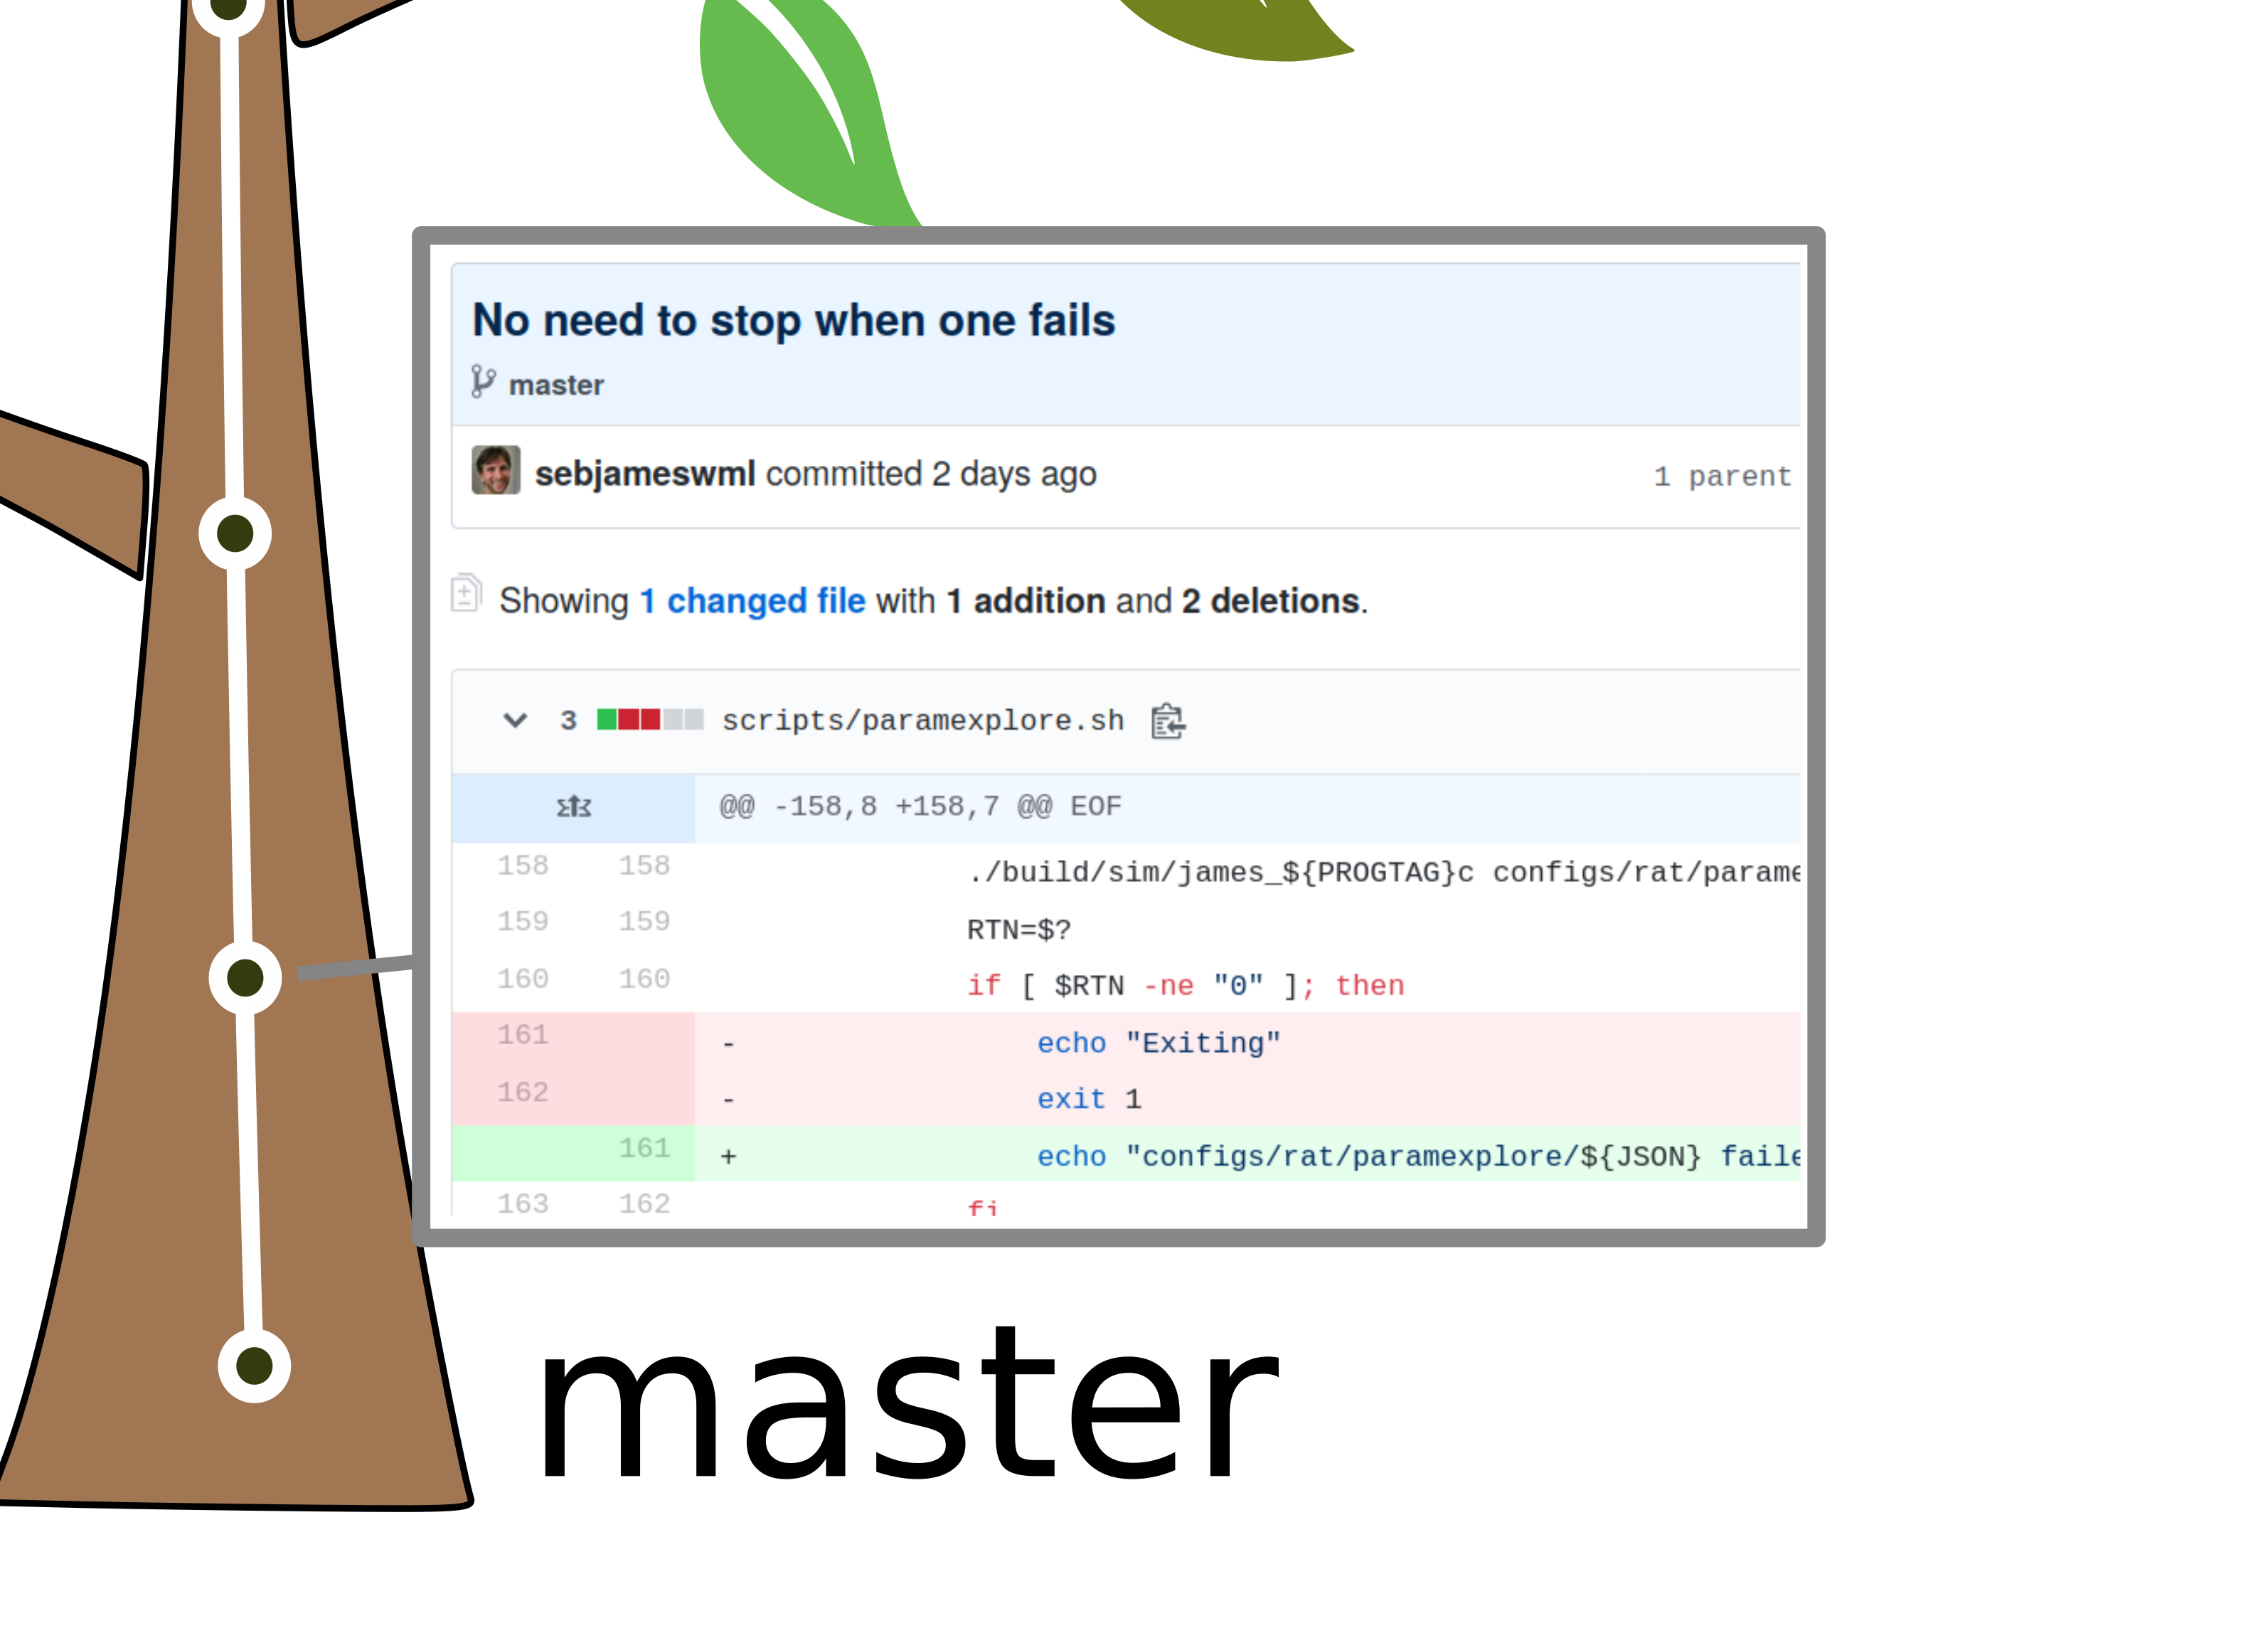
\includegraphics[width=\textwidth]{tree_mastercommits_commitdetail.png}
    \end{column}
  \end{columns}
\end{frame}

% Branch one
\begin{frame}
  \frametitle{Branches instead of file versions}
  \begin{columns}[T]
    \begin{column}{.5\textwidth}
      When you use git, you use \alert{branches} to allow you to experiment with
      different files. There's one central branch, which
      is usually called \textbf{master}.
      \begin{block}{Checkout}
        When you `checkout' a branch, it updates your file to the content it
        has on that particular branch
        \begin{itemize}
          \item Checkout \textbf{idea1}; get myProgram.r with the code for
            your first idea.
          \item Checkout \textbf{NatureNeuroSub1}; get myProgram.r as it was
            when you submitted your paper to Nature Neuroscience.
        \end{itemize}
      \end{block}
    \end{column}
    \begin{column}{.5\textwidth}
      
\includegraphics[width=\textwidth]{tree.png}
    \end{column}
  \end{columns}
\end{frame}

\begin{frame}
  \frametitle{\emph{Project} revisions}
  \begin{itemize}
    \item The ability to branch and tag \emph{really} comes into its own when
      you have any kind of project with more than one file in it.

    \item Without this, you find yourself needing one folder for
      each version of your project, duplicating files left, right
      and centre.
  \end{itemize}

\end{frame}

\begin{frame}
  \frametitle{Working with other people}
  (This is `main feature 2')

  \begin{itemize}
    \item Suppose you have some code which is used by yourself and 5 of your
      colleagues - some sort of library.

    \pause \item You find an error and fix it. Now you have to email the fix to \emph{5} people.

    \pause \item Just after you emailed them, you find an error in your fix, and you
    have to send another email...

    \pause \item Now imagine that one of your colleagues found a
    separate fix in the same file and emails that around. Which fix is
    more important? Who is going to merge the two fixes together?
  \end{itemize}

  \pause You need a revision control system to automate the process of
  distributing changes between users of a set of files, and to manage
  the merging of changes together.
\end{frame}

\begin{frame}
  \frametitle{Other revision control systems}
  \begin{itemize}
  \item RCS (Revision Control System)
  \item SCCS (Source Code Control System)
  \item CVS (Concurrent Versions System)
  \item Subversion
  \item Tons of proprietary systems
  \item Bazaar
  \item BitKeeper
  \item Mercurial
  \end{itemize}

  \pause Git is not the first revision control system, and its
  developers could draw on a lot of collective knowledge when
  designing it.
\end{frame}

\begin{frame}
  \frametitle{Why did someone develop Git?}
  \begin{itemize}
    \pause \item Most revision control tools have been pretty good at
    feature 1 (file versioning)
    \pause \item ...but not great at managing multiple contributions
    \pause \item That caused Linus Torvalds to use the proprietary
    BitKeeper from 2002 to manage the Linux code base.
    \pause \item In 2005 Linus fell out with BitMover Inc., and Git was
    created to replace it.
    \pause \item The name \emph{git} doesn't really mean anything.
  \end{itemize}
\end{frame}

\begin{frame}
  \frametitle{What's different about Git?}
  \begin{itemize}
  \item Git is a \emph{distributed} revision control system
  \pause \item It doesn't have the classical client-server architecture...
  \pause \item ...although typically you will work with a common
  \alert{remote} repository as your \alert{upstream} source.
  \pause \item When you \alert{clone} a repository from a source, you have
    \emph{everything} (all the file history and meta-data) in those
    files to become a source for someone else.
  \pause \item That means you can work on your code, making incremental
  \alert{commits} even when you don't have internet access.
  \pause \item And every copy of the \alert{repo} is a backup!
  \end{itemize}
\end{frame}

\begin{frame}
  \frametitle{Git is \emph{not} github.com}
  \begin{itemize}
  \item Github is a commercial website which makes it easy to use Git
  \item bitbucket.org is an alternative
  \pause \item Generally, public hosting is free, private hosting
  incurs a fee
  \pause \item It's pretty easy to host a git repository yourself, but
  the nice web interface has made github.com very
  popular for source code hosting
  \pause \item It's now a big business; it was acquired by Microsoft in 2018
  \end{itemize}
\end{frame}

\begin{frame}
  \frametitle{Why is Git good for us?}
  We don't have hundreds of people working on the same files, and
  often our work is carried out individually, but...
  \begin{itemize}
    \pause \item We write code, so that's very natural to hold in
    revision control (also XML)
    \pause \item We have a frequent need to \alert{tag} our work (e.g. to
    match up with a paper or document)
    \pause \item ``It used to work, but now I've broken it and I can't
    get it back to working again'': Revision control makes it easy to
    revert to a version of your code which you know will work
    \pause \item You can include your paper alongside your model code
    in a single, public repository
    \item Use of Github is a very effective way to share your
    published models with your peers
  \end{itemize}
\end{frame}

\begin{frame}
  \frametitle{The Git Tutorial}
  The rest of these pages have been put together from material taken
  from the Software Carpentry project, which emphasises the use of
  Git.

  Head over to:

  \url{http://sebjameswml.github.io/git-novice/}

  And start on the lesson ``A better kind of Backup''

\end{frame}

\end{document}
